\chapter{Métricas de evaluación de rendimiento}
 
\section{Introducción}

Este informe presenta una descripción de los variados enfoques y métricas empleados en la actualidad para hacer evaluación de calidad, centrando el análisis en el criterio denominado evaluación objetiva.

No existe actualmente una metodología estandarizada, para hacer una evaluación de la calidad del resultado de de los algoritmos de separación \emph{Foreground} y \emph{Background}.  No obstante, existe un conjunto heterogéneo de métodos de evaluación usados para valorar la calidad de segmentación de un algoritmo. Sin embargo, no existe acuerdo entre los investigadores de usar una metodología de evaluación general, que pueda proporcionar un criterio de comparación común de medición del desempeño. Asimismo, se han puesto a disposición de la comunidad una gran cantidad de escenarios de evaluación ("datasets"), entre estos \cite{singh_muhavi_2010}, que establecen una serie de condiciones (ambientales, iluminación, etc) bajo las cuales, los algoritmos pueden experimentar diversas situaciones para contrastar y evaluar su comportamiento en diferentes situaciones.

Estos métodos han sido clasificados, dependiendo de la naturaleza del evaluador, en diversas metodologías que establecen dos categorías principales; \emph{método de evaluación subjetiva} \cite{mckoen_evaluation_2000} y \emph{método de evaluación objetiva}. Las metodologías de clasificación \emph{subjetiva}, se basan en la valoración que hace un grupo de observadores del resultado final en un proceso de segmentación, pero requiere de un gran número de evaluaciones para producir un resultado con relevancia estadística. En contraste con el método anterior, las metodologías denominadas \emph{objetivas}, buscan una forma de evaluación automática que no requiera la intervención humana en el proceso de medición. En general, el resultado final es una mixtura de métricas, que elaboran un ranking de la calidad de segmentación en una imagen o secuencia de vídeo. Igualmente, el tipo de métricas empleadas en la evaluación objetiva, se dividen en métricas \emph{analíticas} y \emph{empíricas}. Donde las métricas analíticas requiere de conocimiento del algoritmo para evaluar sus requerimientos,  complejidad,  y estructura. Las métricas del tipo empíricas en cambio miden calidad del resultado final de un proceso de segmentación.

Los métodos de evaluación del tipo empíricos se dividen a su vez en métodos de \emph{discrepancia empírica} o \emph{evaluación relativa} y métodos de \emph{evaluación autónomos}. Los métodos de discrepancia se basan en medición de disparidad entre una imagen con anotaciones manuales o de referencia, ``ground truth'', y el resultado de segmentación. Las imágenes con anotaciones manuales funcionan como base de comparación, son mascaras binarias que etiqueta un pixel como background o foreground y tienen como finalidad proporcionar un conjunto de datos independiente y objetivo, con el cual un resultado obtenido puede ser comparado y medido. No obstante, estas mascaras son construidas manualmente, por lo que tienen en forma inherente un cierto grado de error e incertidumbre, que influye en la clasificación final como el mejor resultado que puede ser obtenido. Los métodos autónomos, en cambio, son métodos del tipo \emph{no-supervisados} \cite{zhang_image_2008} donde no requieren una imagen de referencia, evalúan el grado de igualdad de un conjunto de características de imágenes segmentadas previamente determinadas por evaluadores humanos.

Los métodos de evaluación más empleados son los basados en discrepancia empírica, los diferentes modelos propuestos en la literatura plantean una medición objetiva tratando de representar la percepción humana. Las distintas aproximaciones hacen una ponderación del resultado final de acuerdo con la visibilidad de los errores.



\section{Métodos de evaluación de calidad}

Esta parte se enfoca principalmente en métodos de evaluación de calidad basados en \emph{discrepancia empírica}, métodos que hacen una evaluación de percepción de los resultados. En los siguientes párrafos se hace una descripción y análisis de las métricas más recurrentes encontradas en la literatura para hacer evaluación de clasificación de objetos. 

\subsection{Error Cuadrático Medio y Relación a Señal Ruido}

Una de las formas más simples de medir calidad es el \emph{error cuadrático medio} (Median Squared Error - MSE) y la \emph{relación señal a ruido} (Peak Signal-to-Noise - PSNR) \cite{park_benchmark_2013} \cite{park_benchmark_2013}, el cual hace un promedio de el cuadrado de las diferencias de intensidad entre los pixeles de la imagen obtenida y su par de referencia, ground-truh. A pesar que es un método simple de calcular y promediar, ambas mediciones no tienen buena correlación con las medidas de percepción humana.

\begin{equation}
MSE=\frac{1}{N}\sum_{i=1}^N(x_{i}-y_{i})^2
\end{equation}

\begin{equation}
PSNR = 10\log_{10} {\frac{L^2}{MSE}}
\end{equation}

Donde $N$ es el número de pixeles de la imagen, $x_{i}$ e $y_{i}$ es el pixel $i$ de la imagen de referencia y resultante, respectivamente, y $L$ es el rango dinámico del valor de los pixeles. Para 8 bits este valor es 255.
 

\subsection{Métricas de Calidad Estática}
Estas métricas de calidad son elaboradas realizando la comparación individual de un pixel de la imagen resultante con el pixel de su imagen de referencia o ground-truth, es un procedimiento de comparación pixel-pixel. Se utilizan principalmente las medidas de \emph{precision}, \emph{recall} y su media armónica \emph{F-Measure} \cite{brutzer_evaluation_2011} \cite{herrero_background_2009} \cite{park_benchmark_2013}. La variable \emph{recall} es una medida de proporción de pixeles de la imagen de referencia que fueron clasificados correctamente, en cambio, \emph{precision} es una medida de proporción de los pixeles correctos del total de pixeles clasificados.

\begin{equation}
Precision=\frac{total \: pixeles \, en \, foreground \, clasificados \, correctamente}{total \, pixeles \, imagen \, referencia}
\end{equation}

\begin{equation}
Precision=\frac{total \: pixeles \: foreground \, clasificados \, correctamente}{cantidad \, pixeles \, clasificados \, como \, foreground}
\end{equation}



\begin{figure}[!ht]
\centering
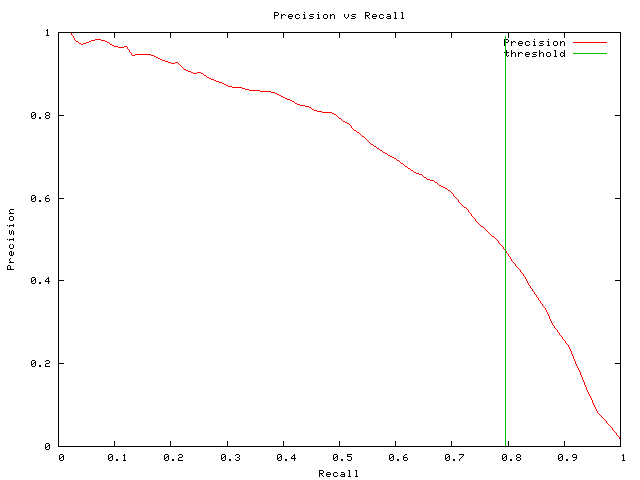
\includegraphics[scale=0.4]{img/prcurve}
\caption{Precision - Recall}
\label{fig:precison versus recall}
\end{figure}


La relación entre ambas variables es un compromiso entre una buena detección (minimizar falso negativos) y buena discriminación (minimizar falso positivos). Estas dos variables ayudan a caracterizar un algoritmo, y en consecuencia a compararlo con otros. Ambos valores son dependientes de los distintos parámetros internos que pueda contener un algoritmo, cualquier ajuste en estos parámetros provoca un cambio en ambas variables y el producto final del algoritmo. De esta manera, se pueden comparar varios algoritmos maximizando el valor de rendimiento global \emph{F-Measure} buscando el mejor compromiso entre \emph{precision}-\emph{recall}.



\begin{equation}
Precision=\frac{TP}{TP+FN}
\end{equation}

\begin{equation}
Recall=\frac{TP}{TP+TN}
\end{equation}

\begin{equation}
F-Measure=\frac{1}{n}\sum_{i=1}^n{2\frac{Precision_{i} \cdot Recall_{i}}{Precision_{i}+Recall_{i}}}
\end{equation}
 
Donde; $TP$ (\emph{verdadero positivo}) es el número de pixeles de un objeto (foreground) correctamente clasificados, $TN$ (\emph{verdadero negativo}) número de pixeles en el background seleccionados correctos, $FP$ (\emph{falso positivo}) número de pixeles pertenecientes al foreground que fueron seleccionados incorrectamente como background, y $FN$ (\emph{falso negativo}) corresponde al número de pixeles de background incorrectamente clasificados como foreground.



\subsection{Métricas de Percepción}

Estas métricas intentan ponderar el concepto de percepción de un observador sobre el resultado final de segmentación, para esto se propone cuantificar \emph{exactitud espacial} (spatial accuracy) y \emph{estabilidad temporal} \cite{liu_metrics_2011} \cite{cavallaro_objective_2002} o \emph{coherencia temporal} \cite{villegas_perceptually-weighted_2004}. Se pondera, mediante algún tipo de función definida, la discrepancia entre una mascara estimada y la de su referencia (ground-truth), tomando en cuenta la inexactitud potencial que puede contener la mascara de referencia, la localización de los pixeles con errores relativo al borde de la mascara de referencia, y el tipo de errores (FP, FN). 

\subsubsection{Contexto espacial y temporal}
El contexto espacial \cite{cavallaro_objective_2002} de un pixel errado es caracterizado por la distancia más cercana de un objeto detectado. Esta propiedad relaciona el foco de atención de un observador hacia a un objeto que le llama la atención, errores del tipo falso negativo (pixel clasificado erróneamente como foreground) son más importantes en la medida que la distancia es mayor. El contexto temporal considera las diferencias de calidad en el tiempo, para esto identifican dos tipos de fenómenos; un efecto sorpresa y un efecto fatiga. El efecto sorpresa se relaciona con los cambios en la exactitud espacial y el efecto fatiga se relaciona con el hecho de un observador se acostumbra a cierto tipo de calidad en el tiempo. Estos dos contextos son relacionados en las siguientes expresiones.

\begin{equation}
\nu_w(n) = 1 - \epsilon_w(n)
\end{equation}

\begin{equation}
\zeta_w(n) = \frac{\nu_w(n)}{2} \lbrack 1 + \alpha_t \frac{d}{dn}\nu(n) \rbrack
\end{equation}

Siendo $\nu_w(n)$ un valor de ponderación de la exactitud espacial, $\frac{d}{dn}\nu(n)$ variación espacial en el tiempo (mientras mayor esta variación más pequeño su coherencia temporal) y $\zeta_w(n)$ una medida de calidad de percepción espacial-temporal. Se define una \emph{exactitud espacial absoluta} y \emph{relativa} (normalización por el total de pixeles) como la contribución de las ponderaciones de $w^i_p$ (falso positivo), y $w^j_n$ (falso negativo) . 

\begin{equation}
w^i_p = \frac{\alpha_p \log(d^i_p + 1)}{D}
\end{equation}

\begin{equation}
w^i_j = \frac{\alpha_nd^j_n}{D}
\end{equation}

\begin{equation}
\epsilon_w() = \sum_{i=1}^{\epsilon_p(n)}w^i_p +	 \sum_{j=1}^{\epsilon_n(n)} w^j_n
\end{equation}


\begin{figure}[!ht]
\centering
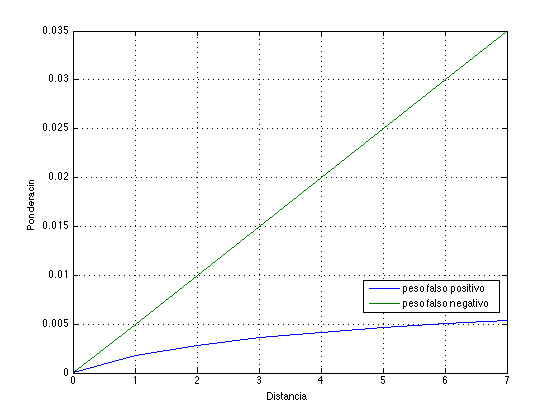
\includegraphics[scale=0.4]{img/PesosFalsoPositivoNegativo}
\caption{Pesos pixeles falso positivo y negativo}
\label{fig:Contexto espacial pesos para pixeles falso positivo y negativo}
\end{figure}

Como se indica en la figura 2, ambas ponderaciones o pesos $w^i_p$ y $w^j_n$ aumentan con la distancia, pero influyen en forma diferenciada en la ponderación final de exactitud espacial. Los pesos para falsos positivos se incrementan en forma lineal, y estos valores son mayores con los pesos de los falsos negativos a la misma distancia.

\subsubsection{Observaciones para cuantificación espacial}

Las mediciones de exactitud espacial en el trabajo propuesto en \cite{liu_metrics_2011}  se basan en observaciones que toman en consideración el error producido al generar las mascaras de referencia en forma manual, se menciona que los pixeles errados muy cerca de los bordes de las mascaras de referencia se presumen son causados por la inexactitud durante la creación de estas mascaras. A su vez, una segunda observación indica que estos mismo errores muy cercanos al borde, tienen poco efecto comparado con otro que se encuentra muy lejano del borde. Pese a que estos pixeles en el borde hacen que un objeto parezca más grueso o delgado, estos no cambian la forma del objeto. Una tercera observación, señala que el impacto de los diferentes tipos de errores durante el procesamiento no son similares, por lo que hacen las distinción de medir en forma independiente falsos negativos y falsos positivos. 

Se propone una función ponderación del tipo sigmoidal, de esta forma errores muy cercanos al borde de la mascara tienen un valor (peso) menor a uno y otros errores lejanos al borde se aproximan a uno. 

\begin{equation}
S(d;\alpha) = \frac{1 - e^{-\alpha \cdot d}}{1 + e^{-\alpha \cdot d}}
\end{equation}

Esta función $S$, tiene como variable $d$ distancia de un pixel en error al borde de la mascara, y $\alpha$ es parámetro que modela la tolerancia de la inexactitud de las mascaras de referencia en sus bordes. Un parámetro $\alpha$ pequeño conlleva una capacidad de tolerancia mayor. 

\begin{figure}[!ht]
\centering
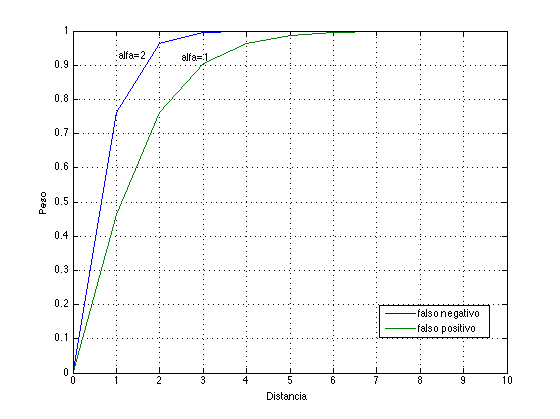
\includegraphics[scale=0.4]{img/sigmoid_function}
\caption{Pesos usando función tipo sigmoidal}
\label{fig:Pesos tipo sigmoidal}
\end{figure}


\subsection{Similaridad Estructural}
El índice de \emph{similaridad estructural} - \emph{SSIM} (Structural SIMilarity) \cite{park_benchmark_2013} \cite{wang_image_2004} es un método de medición de similaridad entre dos imágenes. Es una medida de calidad de una imagen de entrada contrastada con otra de buena calidad. Este índice usa un nuevo enfoque para medir calidad, se basa en la hipótesis que la principal función del ojo humano  es extraer información estructural de su campo visual, y además el Sistema Visual Humano (Human Visual System - HVS) está muy adaptado para realizar esta operación. Por lo tanto una medición de distorsión estructural podría ser una buena aproximación. Se platean entonces, en este nuevo enfoque, moverse desde mediciones de errores (métodos vistos anteriormente) a realizar mediciones de distorsión estructural. Sin embargo, el nuevo problema que se debe enfrentar es cómo definir y cuantificar distorsiones estructurales.

El modo de medir y obtener el índice \emph{SSIM} supone una secuencia de imágenes de entrada en escala de grises además de la secuencia de imágenes de referencia, ground-truth. Se considera la secuencia de referencia como la secuencia con las imágenes de buena calidad, de esta forma la medida de similaridad sirve como una medición de la calidad de la otra secuencia de entrada. La manera de medir similaridad es separar la tarea en tres componentes; \emph{luminancia}, \emph{contraste}, y \emph{estructura}.

\begin{equation}
SSIM(x,y) = f(l(x,y), c(x,y),s(x,y)) 
\end{equation}

\begin{equation}
SSIM(S,G) = (\frac{2\mu_S\mu_G + c_1}{\mu_S^2 + \mu_G^2 + c_1}) \cdot (\frac{2\sigma_S\sigma_G + c_2}{\sigma_S^2\sigma_G^2 + c_2}) \cdot (\frac{\mu_{SG} + c_3}{\mu_S\mu_G + c_3})
\end{equation}

Este índice de calidad es una combinación de tres factores, pérdida de correlación, distorsión media, y varianza de la distorsión. El primer componente es el coeficiente de correlación lineal entre $S$ y $G$ y su rango dinámico varia en $[-1,1]$. El segundo componente mide similaridad entre valores medios, y su rango de valores está entre $[0,1]$. El tercer componente mide similaridad entre las varianzas de ambas imágenes de una secuencia, y su rango dinámico está entre $[0,1]$. La relación final aplicada sobre secuencia de vídeo viene dada por la siguiente formula. 


\begin{equation}
SSIM(S,G) = \frac{1}{n} \sum_{i=1}^{n} \frac{(2\mu_{S_{i}} \mu_{G_{i}} + c_1) \cdot (2 cov_{S_iG_i} + c_2)}  {(\mu^2_{S_i} + \mu^2_{G_i} + c_1) \cdot (\sigma^2_{S_i} + \sigma^2_{G_i} + c_2)}
\end{equation}

Donde, $S$ es un conjunto de $n$ imágenes resultantes, $G$ conjunto de las imágenes de referencia (ground-truth), $\mu_{S_i}$ $\mu_{G_i}$ media de ambas secuencias, $\sigma_{S_i}$ y $\sigma_{G_i}$ desviaciones estándar, y $cov_{S_iG_i}$ covarianza de $S_i$ y $G_i$. Las constantes $c_1 = (k_1 + L)^2$ $c_2=(k_2 + L)^2$ con valores $k_1=0.01$ $k_2=0.03$ y $L=255$.


\subsection{D-Score}
D-Score brinda un criterio de \emph{disimilitud} entre una imagen de referencia y la imagen de entrada, esta métrica sólo considera fallas en la medición de los resultados. El costo de un error depende de la distancia con el objeto más cercano de la referencia, teniendo una ponderación mayor los errores en el rango intermedio. Esto debido que este tipo de errores impactan de mayor manera el reconocimiento de formas. Por ende, errores en zonas lejanas/cercanas tendran un D-score cercano a cero. 

\begin{equation}
DT(x) = min( d(p,x), \forall x \in X)
\end{equation}

El costo de error se basa en una \emph{Tranformada de Distancia} (Distant Transform - DT) de la referencia ground-truth, con $X$ un conjunto de pixeles de referencia, $d(p,x)$ es la distancia del pixel $p$ al pixel $x$, entonces $DT(x)$ es la distancia mínima entre un pixel $x$ y el punto de referencia más cercano. Para calcular $DT(x)$ se usa la siguiente relación

\begin{equation}
D-score(x) = exp( - (\log_2(2.DT(x)) - \alpha )^2)
\end{equation}


\begin{figure}[!ht]
\centering
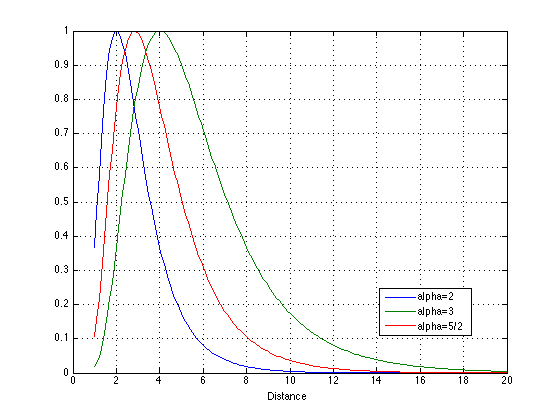
\includegraphics[scale=0.4]{img/dscore}
\caption{Valores D-Score basados en la distancia desde la referencia ground-truth}
\label{fig:Valores D-Score}
\end{figure}

De acuerdo con la figura 4, se tiene una tolerancia de 3 pixeles desde la referencia, esto debido que ese tipo de errores locales no afecta realmente el proceso de reconocimiento. De esta misma forma tomando un valor de $\alpha=5/2$, \cite{park_benchmark_2013}, se permiten que ocurran errores a más de 10 pixeles de distancia. D-score entrega un índice que señala el nivel de reconocimiento de objetos, en la medida que este valor es menor, mejor es el reconomiciento, independiente del valor de errores que entreguen otros índices, como el \emph{F-Measure}.

\subsection{Conclusiones}
Se ha hecho una descripción de la mayoría de los métodos de medición utilizados actualmente, basados principalmente en el paradigma de evaluación por discrepancia  o error. Donde la menor discrepancia con una referencia brindan un ranking de mayor calidad en proceso de clasificación o comparación de algoritmos. Se puede señalar que en general no existe una métrica ideal que pueda ser utilizada como herramienta de comparación universal en los diferentes algoritmos existentes. De igual modo, estas pueden ser empleadas en conjunto de forma complementaría aprovechando las diferentes características de ellas. Un caso concreto es el trabajo desarrollado para el desafío BMC \cite{park_benchmark_2013}.

Las metricas más empleadas sin duda son ``precision'', ``recall'' y todas sus demás variantes, estas métricas son una orientación para distinguir buena detección de una buena clasificación, usando ambas de manera complementaria; se puede obtener una alta ``precision'' con un bajo ``recall'', es decir, se puede tener una buena tasa de detección pero baja discriminación de objetos. En consecuencia, son un compromiso entre ellas, compromiso que es logrado con el máximo valor de la métrica de rendimiento ``F-Measure''. 

Las diferentes métodos basadas en el concepto de percepción se aproximan a una forma de evaluación que podría hacer un observador humano, para esto, hacen una combinación de un contexto espacial con un contexto temporal. Los errores se ponderan de acuerdo con distancia al borde de la mascara de referencia, la estabilidad de esta percepción espacial es además considerada en la evaluación de calidad. Los distintos enfoques encontrados de esta metodología se diferencian en el tipo de función empleada para hacer la ponderación espacial de los errores con respecto a la distancia del borde de su mascara. Evalúan con mayor ponderación el error falso negativo y localizado lejano al borde de la mascara. La métrica de ``D-Scorre'', a diferencia de la descripción previa castiga fuertemente los pixeles errados en el borde de la mascara, porque este tipo de errores no permiten realizar una buena clasificación.

Un diferente enfoque presenta el índice de similaridad, este ya no utiliza las mediciones de percepción para evaluar calidad. Postula medición de distorsión estructural, para esto se propone una combinación de mediciones de luminancia, contraste y estructura. Que vienen siendo análisis de correlación entre dos imágenes, cuantificación de sus varianzas y sus medias. 

Finalmente, estas distintas métricas pueden ser empleadas en conjunto o en forma individual. Pero una combinación de ellas podría brindar una mejor claridad desde el punto de vista de la calidad de los diferentes algoritmos. Pueden entregar una mejor discriminación de las ventajas y falencias en diversas condiciones ambientales. Se podría determinar un buen algoritmo para ciertas condiciones, pero también determinar sus desventajas en otras situaciones. 

Se propone de esta forma utilizar la herramienta del desafio BMC \cite{park_benchmark_2013}, para hacer evaluación de calidad del algoritmo de sustracción de imágenes.
 
 




